\documentclass[../main]{subfiles}
\begin{document}

\graphicspath{{../figures}}

\section{実験結果・考察}
まず,正常音のマッピングによる経路内における異常判別結果を示す.
\reffig{energy_normal}に示すように,正常音のデータに対しては,経路内の全ての座標において,観測音と正常音の差分エネルギーが経路を通じて極めて小さいことが確認できる.
一方で異常音源の存在する環境下では\ref{energy_abnormal}に示すように,異常音源を設置した(0.5m, -0.3m)付近の経路においてエネルギーが急激に増加していることが確認できる.
これらから,ニューラルネットワークを用いた正常音のマッピングによる異常の判別が可能であることが確かめられた.

次に,異常音源の座標推定結果を示す.
表\ref{tab:result}に示すように,異常音源の座標を精度よく推定できていることが確認できる.

異常音源の座標を精度よく推定できた原因として,実験設定において異常音源のエネルギーが正常音のエネルギーと比較して大きかったことが挙げられる.
異常音源のエネルギーが小さい場合にも同様に異常音源の座標を精度よく推定できるようにすることが今後の課題として挙げられる.

\begin{figure}[tb]
  \centering
  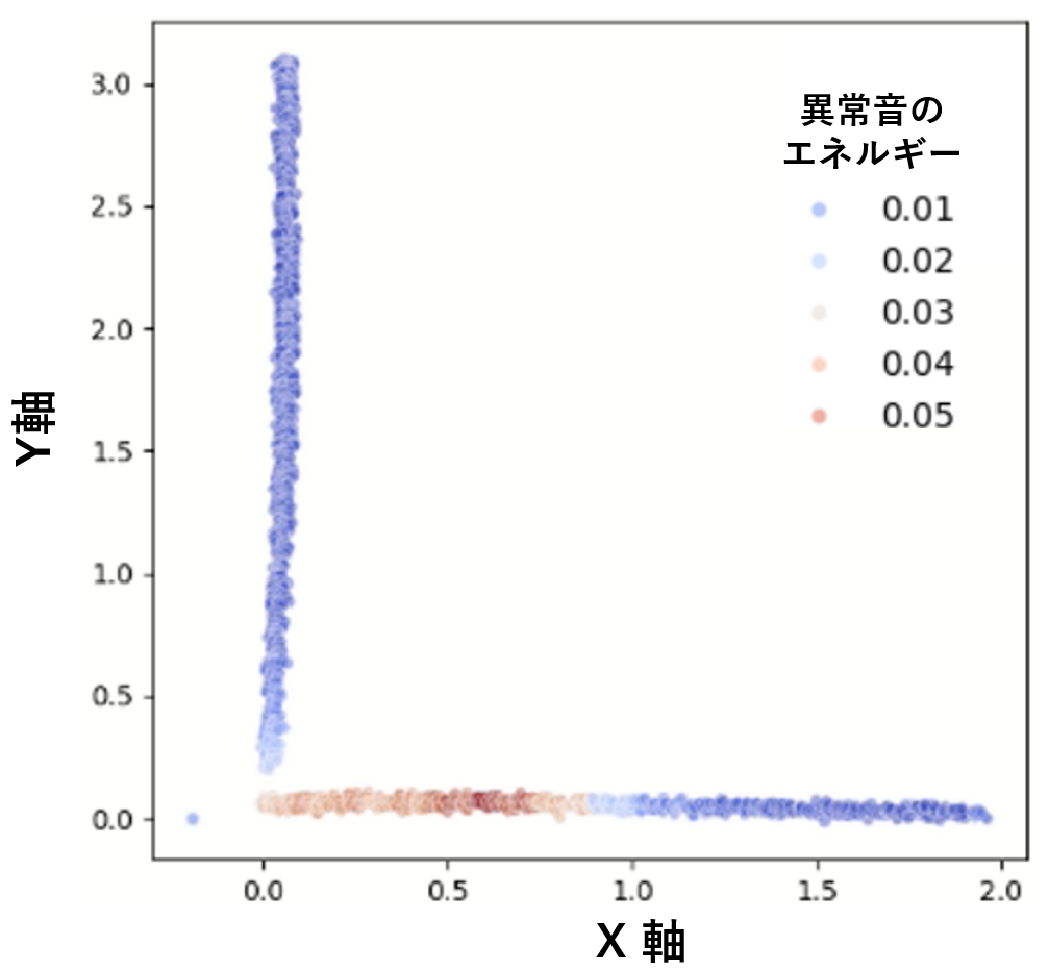
\includegraphics[keepaspectratio, width=0.8\linewidth]{energy_normal.pdf}
  \caption{正常データにおける経路上の異常音のエネルギー}
  \labfig{energy_normal}
\end{figure}


\begin{figure}[tb]
  \centering
  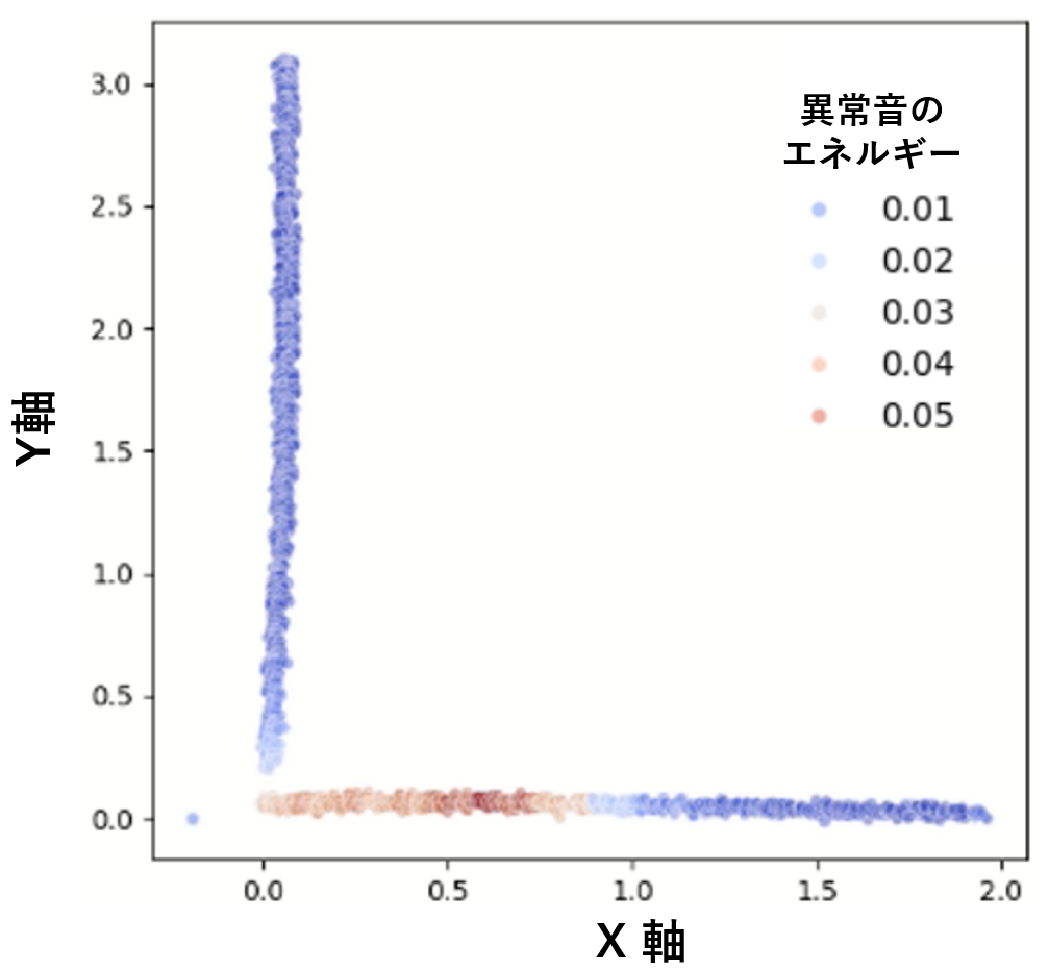
\includegraphics[keepaspectratio, width=0.8\linewidth]{energy_abnormal.pdf}
  \caption{異常データにおける経路上の異常音のエネルギー}
  \labfig{energy_abnormal}
\end{figure}

\begin{table}[h]
  \centering
  \begin{tabular}{|c|c|}
  \hline
  真値 & (0.50, -0.30) \\ \hline
  推定値 & (0.53, -0.31) \\ \hline
  \end{tabular}
  \caption{異常音源の座標推定結果 (x 座標, y 座標)}
  \label{tab:result}
\end{table}


\end{document}
